\chapter{Project Loom}
\label{cha:ProjectLoom}

    Projekt Loom wurde 2017 von Ron Pressler ins Leben gerufen und ist ein Open-Source-Projekt, 
    das sich auf die Verbesserung der \gls{jvm} konzentriert. Das Ziel von Project Loom ist es, 
    die \gls{jvm} so zu erweitern, dass der Aufwand für das Schreiben, Warten und Überwachen von hochdurchsatzfähigen nebenläufigen Anwendungen,
    die die verfügbare Hardware optimal nutzen, drastisch reduziert wird \cite{ProjectLoom}.

    Die wichtigste Neuerung sind \emph{\Glspl{vt}}.
    Diese virtuellen Threads sind Threads, die im Gegensatz zu \Glspl{pt} von der JVM verwaltet werden und nicht direkt vom Betriebssystem. 
    Sie sind leichtgewichtiger als normale Threads, da sie weniger Speicher benötigen und schneller erstellt werden können \cite{JEP444}.
    Virtuelle Threads sind auch als "Continuations" bekannt und werden in anderen Programmiersprachen wie Python, Ruby und JavaScript verwendet.
    Project Loom soll die JVM so erweitern, dass sie virtuelle Threads unterstützt und Entwicklern eine einfachere Möglichkeit bietet,
    nebenläufige Anwendungen zu erstellen. Virtuelle Threads sollen die Leistung von Java-Anwendungen verbessern, indem sie die Anzahl der \Glspl{pt} reduzieren und 
    die Verwaltung von Threads vereinfachen. 

    Aufbauend darauf wird auch \emph{Strukturierte Nebenläufigkeit (Structured Concurrency)} vorgestellt.
    \texttt{StructuredTaskScope}s sollen eine Gruppe von Threads, die parallel ausgeführt werden, aber verwandte Aufgaben erledigen, als eine Arbeitseinheit behandeln. 
    Dabei soll keine Sicherheit oder Kontrolle über die einzelnen Aufgaben eingebüßt werden, sondern Kontrolle über das Gesamtverhalten der Gruppe gewonnen werden.
    Dies soll eine parallele Ausführung von verschiedenen Aufgaben einfacher gestalten und die Fehlersuche erleichtern.
    Im Hintergrund kommen dafür \Glspl{vt} zum Einsatz \cite{JEP453}.

    \emph{Bereichsgebundene Werte (Scoped Values)} sind Werte, deren Gültigkeitsbereich nach Belieben festgelegt werden kann.
    Auch Verschachtelungen der Bereiche oder das
    Zuweisen verschiedener Werte auf verschiedenen Threads, ähnlich zu \texttt{ThreadLocal<>}, sind möglich. Ihre Effizienz wurde auf \Glspl{vt} optimiert
    \cite{JEP481}.
    Project Loom ist ein laufendes Projekt und manche Funktionalitäten sind noch als Preview-Funktionalität eingestuft und können in späteren Versionen Änderungen 
    unterzogen werden oder sogar wieder entfernt werden.



\section{Virtuelle Threads}                                 % 5 Seiten ---------------------------------------------------------------------------------------------------------
\label{sec:VirtuelleThreads}

Virtuelle Threads sind die das Herzstück von Projekt Loom und eine neue Funktion in der Java Virtual Machine (JVM), die es ermöglicht, Millionen von Threads effizient zu verwalten.
Sie sind leichtgewichtig und bieten eine bessere Skalierbarkeit für nebenläufige Anwendungen.
\Glspl{vt} entlasten Entwickler von der Komplexität der Thread-Verwaltung und verbessern die Performanz von Anwendungen erheblich.


\subsection{Was sind Virtuelle Threads?}
\label{subsec:WassindVTs?}

    Im Gegensatz zu dem bisherigen Threadmodell von Java hängt die Implementierung von \Glspl{vt} nicht so stark von den \Glspl{ot} ab. Sie führen zwar noch Code 
    auf diesen aus aber binden diesen nicht mehr ihre gesamte Lebenszeit lang an sich, im Gegensatz zu den herkömmlichen \Glspl{pt}. Dies hat zur Folge, 
    dass mehrere \Glspl{vt} Aufgaben zeitversetzt auf ein und demselben \gls{ot} ausführen können und die maximale Anzahl der \Glspl{vt}
    die maximale Anzahl von \Glspl{ot} wesentlich überschreiten kann.
    Virtuelle Threads werden aber nicht direkt auf OS Threads aufgesetzt, sondern auf Plattform Threads.
    Daher werden diese auch oft als "Carrier Threads" bezeichnet \cite{ieee2022}.
    

    \begin{figure}[H]
        \centering
        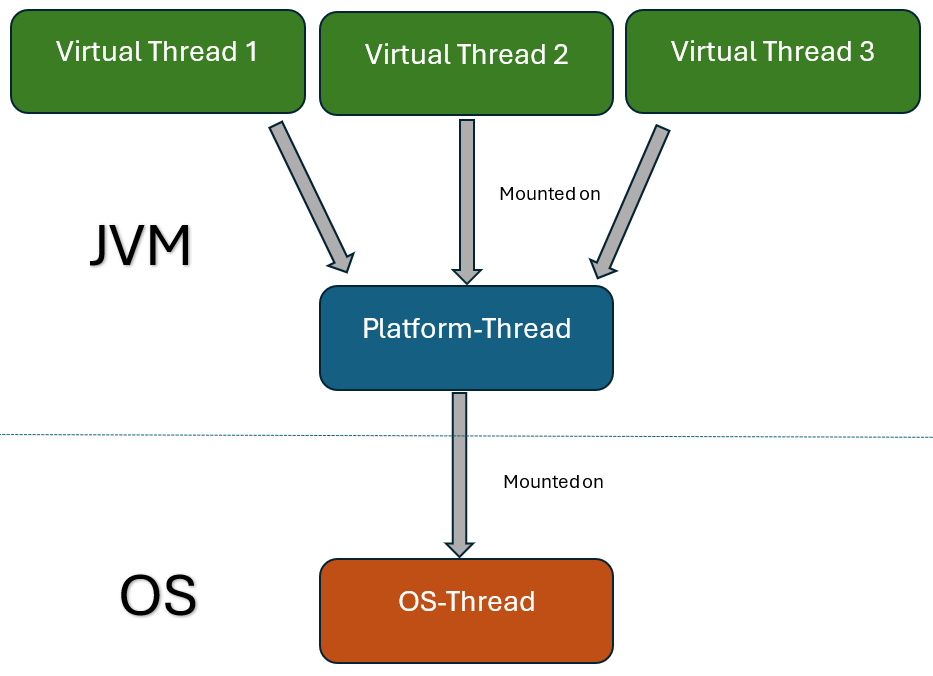
\includegraphics[width=0.6\textwidth]{VTs}
        \caption{Virtuelle Threads in der JVM}
        \label{fig:VTs}
    \end{figure}

    Da \Glspl{vt} vollkommen von der \gls{jvm} verwaltet werden und diese über die Art von Aufgabe und derzeitigen Zustand des Threads Bescheid weiß, kann die
    \gls{jvm} einen \gls{vt} von dem ihm zugeteilten \gls{pt} temporär lösen und einen anderen \gls{vt} darauf Code ausführen lassen, da das Blockieren von \Glspl{vt}
    sehr billig ist. Dies hat zur Folge, dass \Glspl{vt} nur dann Rechenzeit erhalten, wenn sie auch benötigt wird. Somit wird der Durchsatz an Recheninstruktionen
    eines \gls{pt} stark erhöht.
    Wird aber nur ein einzelner Thread benötigt, können diese Vorteile nicht genutzt werden. Der \gls{pt}, dem der \gls{vt} zugewiesen wurde, bindet den \gls{ot} auch
    an sich, selbst wenn kein \gls{vt} Code ausführt \cite{JEP444}.
    

    \begin{figure}[H]
        \centering
        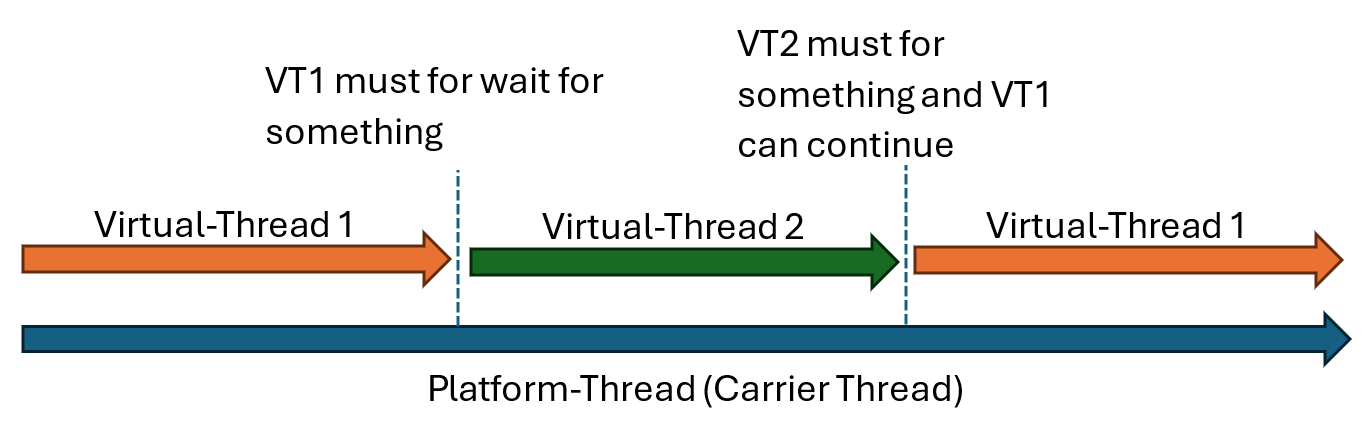
\includegraphics[width=0.67\textwidth]{VT_Coroutine}
        \caption{Coroutine von \Glspl{vt}}
        \label{fig:VT_Coroutine}
    \end{figure}

    Die \gls{jvm} kann auch die initiale Ressourcenzuweisung bei \Glspl{vt} viel präziser durchführen als das Betriebssystem bei \Glspl{ot}, die mit jedem neuen \gls{pt}
    erstellt werden. Durch die enge Bindung eines \Glspl{pt} an seinen \gls{ot} wird der Speicher für den Stack bei der Erstellung des Threads festgelegt.
    Eine dynamische Veränderung der Größe wird nicht unterstützt. Übersteigt die benötigte Größe des Stacks die Vorgaben der \gls{jvm}, wird ein \texttt{StackOverflowError}
    geworfen \cite{jvmSpecification}. Diese initiale Größe kann mit der Option \texttt{-Xss<stack-size>} für die Ausführung der \gls{jvm} verändert werden -- wobei 
    je nach Betriebssystem und \gls{jvm} auch hier Einschränkungen gelten -- oder im Konstruktor des Threads mitgegeben werden.
    Da das Betriebssystem nicht weiß, wie spezifische Programmiersprachen ihren Stack verwalten, allokiert
    es den Speicher für den Stack eher großzügig \cite{ProjectLoom}.
    \Glspl{vt} hingegen speichern ihren Stack als sogenannte "stack chunk object" am Heap ab. Natürlich muss der Stack bei einem Kontextwechsel vom Heap auf den \gls{pt} kopiert werden und umgekehrt. Dieser
    Vorgang verursacht einen gewissen Overhead, der aber durch andere Verbesserungen kompensiert wird.
    Diese können zur Laufzeit wegen ihrer losen Bindung zu \Glspl{ot}
    dynamisch ihre Größe ändern. Eine wesentliche Herausforderung bei der Umsetzung von Projekt Loom war die Anpassung der Garbage-Kollektoren.
    Im Gegensatz zu \Glspl{pt} sind \Glspl{vt} auch keine "GC-Roots", also Startobjekte für den Speicherfreigabe-Prozess. Alle nicht durch GC-Roots erreichbaren
    Objekte werden vom "Garbage Collector" freigegeben. Dadurch werden die in \Glspl{vt} enthaltenen
    Referenzen nicht immer vom Garbage Collector durchwandert. Wird beispielsweise ein \gls{vt} durch ein \texttt{BlockingQueue.take()} blockiert und es besitzt kein anderer Thread eine
    Referenz auf den \gls{vt} oder die \texttt{BlockingQueue}, wird der \gls{vt} freigegeben. Dies ist erwünschtes Verhalten, da dieser in diesem Fall 
    nicht wieder entblockt werden kann. Würde das nicht passieren, spräche man von einem "Thread-Leck" -- einem Thread der nutzlos im Hintergrund ausgeführt wird und somit
    Systemressourcen verschwendet. 
    Sollte der \gls{vt} aber laufen oder ein anderer Thread eine Referenz auf die \texttt{BlockingQueue} enthalten, ist der 
    \gls{vt} über die GC-Root des \gls{pt} erreichbar und bleibt bestehen \cite{JEP425}.
    Vor allem bei Anwendungen, die viele Threads über einen längeren Zeitraum  laufen lassen, trägt das Verhalten von \Glspl{vt} zur Effizienz und Stabilität bei.
    Ansonsten unterscheiden sich \Glspl{vt} nicht stark von \Glspl{pt} und werden von den gleichen Problemen  wie beispielsweise Deadlocks und Race Conditions geplagt \cite{JEP425}.
% Thread leaks + warum sie bei vts weniger häufig auftreten und warum ewig blockierte vts nicht ganz so schlimm sind 

\subsection{Wie werden VTs benutzt?}
\label{subsec:WieWerdenVTsBenutzt?}

    Die Erstellung und Verwendung von virtuellen Threads unterscheidet sich nicht stark von den Platform-Threads. 
    \begin{program} [H]
        \caption{Erstellung eines \Glspl{vt}}
        \label{prog:ErstellungEinesVT}
    \begin{JavaCode}[language=Java, numbers=left]
public static void main(String[] args) {
    Thread vt = Thread.ofVirtual().name("VirtualThread").unstarted(() -> {
        System.out.println("Hello from a virtual thread!");
    });
    vt.setPriority(Thread.MAX_PRIORITY);
    vt.start();
    Thread vt1 = Thread.startVirtualThread(() -> {
        System.out.println("Hello from another virtual thread!");
    });
    try {
        vt.join(); vt1.join();
    } catch (InterruptedException e) {
        e.printStackTrace();
    }
}\end{JavaCode}
    \end{program}
    Anstatt \texttt{new Thread(Runnable task).start();} wird der Ausdruck aus Zeile 2 in Programm 
    \ref{prog:ErstellungEinesVT} benutzt, um einen neuen virtuellen Thread zu erstellen. Dabei kann der \texttt{unstarted} Methode ein \texttt{Runnable} mitgegeben werden, um den Thread später mit 
    \texttt{start} zu starten. Alternativ kann auch ohne der 
    \texttt{unstarted} Methode \texttt{.start(Runnable r)} aufgerufen werden, um den Thread sofort zu starten. 
    Analog dazu wurde die die Factory-Methode \texttt{ofPlatform(Runnable task)} zur Erstellung von \Glspl{pt} hinzugefügt um die Schnittstellen konsistenter zu gestalten.
    Sollte ein \gls{vt} sofort gestartet werden, kann auch \texttt{startVirtualThread} 
    wie in Zeile 7 benutzt werden. Diese Methode nimmt ebenfalls ein
    \texttt{Runnable} als Parameter. \texttt{Thread.join()} lässt genauso wie bei \Glspl{pt} den aktuellen Thread 
    auf die Beendung des Threads warten, für den \texttt{.join()} aufgerufen wurde. Die Nachteile dieser Art der Verwendung sind Codeduplizierung und erhöhter Aufwand
    beim Starten mehrerer Threads, da Eigenschaften wie der Name für jeden Thread individuell angepasst werden müssen. Typische Anwendungsfälle sind schnelle
    einmalige Aufgaben, die sofort und ohne umfangreiche Konfigurationen ausgeführt werden sollen \cite{oracle21Thread}.
    % beispiel für einen Vt mit return wert über eine FutureTask<>

    \begin{program} [H]
        \caption{\Glspl{vt} mit Rückgabewert}
        \label{prog:VTMitRückgabewert}
    \begin{JavaCode}[language=Java, numbers=left]
public static void main(String[] args) {
    FutureTask<String> futureTask = new FutureTask<>(() -> {
        Thread.sleep(1000);
        return "Task completed";
    });
    Thread.ofVirtual().start(futureTask);
    try {
        System.out.println(STR."Result: \{futureTask.get()}");
    } catch (Exception e) {
        e.printStackTrace();
    }
}\end{JavaCode}
    \end{program}
    Sollte der auszuführende Code einen Rückgabewert liefern, kann wie in Programm \ref{prog:VTMitRückgabewert} in Zeile 6 dem Thread eine \texttt{FutureTask<>} mitgegeben werden. Diese nimmt wiederum
    ein \texttt{Callable<>}, das im Gegensatz zum \texttt{Runnable} einen Wert retourniert. Das Ergebnis kann -- wie in Zeile 8 -- mit der Methode \texttt{get()} abgefragt werden.
    Diese Methode wartet auf das Ergebnis indem sie den Eltern-Thread blockiert und somit das \texttt{join()} ersetzt.



    Weiters besteht auch die Möglichkeit, einen \texttt{Thread.Builder} zu benutzen, der die Anpassung solcher Eigenschaften wie eine Zeichenkette und fortlaufende Zahl
    als Name selbständig weiterführt.
    Bei \Glspl{pt} verändert \texttt{.setPriority(int)} je nach Betriebsystem und Implementierung der \gls{jvm} die Priorität des Threads im Prozess-Scheduler. Bei \Glspl{vt} ist dieser Methodenaufruf in Java 21 zwar
    möglich, hat aber keine Auswirkungen, da die Priorität auf \texttt{NORM\_PRIORITY} fixiert wurde. Dies könnte sich aber in zukünftigen Versionen ändern \cite{JEP444}.

    
    
    \begin{program} [H]
        \caption{Beispiel eines \texttt{Thread.Builder} für \Glspl{vt} in Java}
        \label{prog:ErstellungEinesVTBuilders}
    \begin{JavaCode}[language=Java, numbers=left]
public static void main(String[] args) {
    try {
        Thread.Builder builder = Thread.ofVirtual().name("worker-", 0);
        Runnable task = () -> {
            // do something
        };
        // name "worker-0"
        Thread t1 = builder.unstarted(task);
        t1.setPriority(Thread.MAX_PRIORITY);    //Priority is set for each Thread 
                                                //individually   
        t1.start(); t1.join();
        System.out.println(t1.getName() + " terminated");
        // name "worker-1"
        Thread t2 = builder.start(task);   
        t2.join();  
        System.out.println(t2.getName() + " terminated");
    } catch (InterruptedException e) {
        e.printStackTrace();
    }
}\end{JavaCode}
    \end{program}

    Dabei können Regeln für verschiedene Attribute wie eine Namenskonvention
    in einem Schritt für alle späteren Threads festgelegt werden, was Codeduplizierung entgegenwirkt.
    Die Methode \texttt{name(String, long)} ermöglicht eine automatisierte fortlaufende Benennung zukünftig erstellten Threads. Wie wie in Zeile 3 in Programm 
    \ref{prog:ErstellungEinesVTBuilders} zu sehen ist, nimmt die Methode einen Präfix in Form einer Zeichenkette und einen Startwert vom primitiven
    Datentypen \texttt{long}. Der erste durch den Builder erstellte Thread bekommt als Namen eine Konkatinierung des Präfixes und des Startwertes. Bei jedem weiteren Thread wird der Startwert um eins inkrementiert. Lässt man den Startwert als Methodenparameter weg, heißen alle Threads gleich 
    \cite{oracle22Builder}. 

    \begin{program} [H]
        \caption{Beispiel eines \texttt{newVirtualThreadPerTaskExecutor()} in Java}
        \label{prog:ErstellungEinesExecutors}
    \begin{JavaCode}[language=Java, numbers=left]
public static void main(String[] args) {
    try (var executor = Executors.newVirtualThreadPerTaskExecutor()){
        IntStream.range(0, 1000).forEach(i -> {
            executor.execute(() -> {     
                /* .submit() returns a Future<> object that can be used to retrieve
                 the result of a computation; .execute() does not return a result.*/
                System.out.println("Thread " + i + " started");
            });
        });
    }       /* executor.close() is called is called implicitly and the Thread waits
             for all tasks to finish */
    System.out.println("All Tasks finished"); 
}\end{JavaCode}
    \end{program}

    Wird eine große Anzahl an \Glspl{vt} benötigt,  ist ein Executor bzw. Threadpool empfehlenswert. Dieser sollte in Kombination mit einem
    try-with-resources-Block verwendet werden, da dieser beim Verlassen des Blockes implizit geschlossen wird. Wird dies nämlich nicht gemacht, kann es
    im Falle einer Ausnahme dazu kommen, dass ein Thread nicht beendet wird und so als Thread-Leck weiterhin im Hintergrund Systemressourcen verschwendet.
    Der \texttt{ExecutorService} der mit der statischen Fabrikmethode \texttt{.newVirtualThreadPerTaskExecutor()} erstellt wird, 
    erstellt im Gegensatz zum herkömmlichen \texttt{ExecutorService} für jede Aufgabe einen neuen \gls{vt}. Die Instanziierung und Verwendung eines solchen \texttt{ExecutorService} 
    ist in Programm \ref{prog:ErstellungEinesExecutors} in Zeile 2 zu sehen.
    Sollten die Aufgaben einen Wert retournieren, muss anstatt \texttt{execute} die Methode \texttt{submit} benutzt werden. Dies liefert ein \texttt{Future<T>}-Objekt 
    \cite{oracle21VritualThreads}.
    Der von der \texttt{Future} enthaltene Wert kann mit der
    \texttt{get()}  Methode ausgelesen werden. Dabei handelt es sich um eine blockierende Instruktion. Daher wird die Ausführung des Eltern-Threads bis zur
    Beendung des Kind-Threads angehalten \cite{oracle21Future}.
    


\section{Structured Concurrency}                                 % 4 Seiten ---------------------------------------------------------------------------------------------------------
\label{sec:Structured Concurrency}

    Structured Concurrency (strukturierte Nebenläufigkeit) ist ein Programmierkonzept, das darauf abzielt, die Handhabung von nebenläufigen Aufgaben zu vereinfachen und sicherer zu machen.
    Es stellt sicher, dass alle gestarteten Aufgaben innerhalb eines bestimmten Bereichs abgeschlossen werden, bevor dieser verlassen wird.
    Dies führt zu besser lesbarem und wartbarem Code und reduziert die Wahrscheinlichkeit von Fehlern.

\subsection{Was ist Structured Concurrency?}
\label{subsec:WasistSC?}
    \emph{Strukturierte Nebenläufigkeit (Structured Concurrency)} in Project Loom fügt die Klasse \texttt{\gls{sts}} und 2 Ableitungen davon zur Standartbibliothek von Java hinzu
    und befindet sich derzeit noch in
    aktiver Entwicklung. Das heißt, dass sich verschiedene Funktionalitäten ändern oder wieder entfernt werden können.
    Die zu strukturierten Nebenläufigkeit gehörigen Klassen ermöglichen
    es, eine Gruppe von parallelen Teilaufgaben als eine Einheit zu koordinieren. Allgemeine Ausführungslogik und Fehlerbehandlung kann dadurch schon vorher festgelegt und 
    wiederverwendet werden.
    Wie der Name bereits verrät, wird dabei ein Block festgelegt, in dem diese Teilaufgaben erstellt und behandelt werden.
    Dadurch müssen die Teilaufgaben vor dem Thread, in dem sie gestartet wurden, beendet werden \cite{oracle21SC}.

    \begin{program} [H]
        \caption{Beispiel für einen einfachen \gls{sts}}
        \label{prog:BeispielFürEinenEinfachenSts}
    \begin{JavaCode}[language=Java, numbers=left]
public static void main(String[] args) {
    try (var scope = new StructuredTaskScope<>()) {
        StructuredTaskScope.Subtask<String> result1 = scope.fork(() -> {
            Thread.sleep(1000);
            return "Result from task 1";
        });
        StructuredTaskScope.Subtask<Boolean> result2 = scope.fork(() -> {
            Thread.sleep(2000);
            throw new RuntimeException("Task 2 failed");
        });
        StructuredTaskScope.Subtask<Integer> result3 = scope.fork(() -> {
            Thread.sleep(3000);
            return 3;
        });
        scope.join();                        // Waits for all subtasks to complete
        if (result1.state() == StructuredTaskScope.Subtask.State.SUCCESS){
            System.out.println(result1.get());  
        } 
        System.out.println(result2.get());   // Throws an IllegalStateException
        System.out.println(result3.get());
    } catch (Exception e) {                  // calls .close() implizit.
        e.printStackTrace();
    }
}\end{JavaCode}
    \end{program}
    Wird der \gls{sts} ohne Typ erstellt, können die einzelnen Teilprozesse Objekte verschiedener Typen retournieren. Der Ausdruck \texttt{new StructuredTaskScope<Integer>()}
    hätte beispielsweise eine einschränkende Wirkung.
    Es wird stark empfohlen, einen \gls{sts} in Form eines try-with-resources-Blocks zu realisieren, da dieser den Gültigkeitsbereich wieder schließt. In diesem Block
    werden Teilaufgaben mit der Methode \texttt{.fork(Runnable r)} erschaffen. Dieser Vorgang kann in Programm \ref{prog:BeispielFürEinenEinfachenSts} in den Zeilen 3, 7 und 11 beobachtet werden.
    Diesen Teilaufgaben haben den Rückgabewert \texttt{StructuredTaskScope.Subtask<T>}, wobei sie keine
    primitiven Datentypen aufnehmen können. Mit \texttt{.state()} kann überprüft werden, ob die einzelnen Ausführungen erfolgreich waren.
    Wichtig dabei ist der Aufruf von \texttt{.join()}. Dadurch wartet der \gls{sts} darauf, dass entweder alle Teilprozesse beendet werden oder
    fehlschlagen, oder
    eine andere vordefinierte Abbruchbedingung erreicht wird. Außerdem garantiert dieser Aufruf die Freigabe sämtlicher virtuellen Threads \cite{oracle21STS}.
    

    \begin{program} [H]
        \caption{Beispiel für \texttt{ShutdownOnFailure}}
        \label{prog:BeispielFürShutdownOnFailure}
    \begin{JavaCode}[language=Java, numbers=left]
public static void main(String[] args) {
    StructuredTaskScope.Subtask<String> result1 = null;
    StructuredTaskScope.Subtask<String> result2 = null;
    StructuredTaskScope.Subtask<String> result3 = null;
    try (var scope = new StructuredTaskScope.ShutdownOnFailure()) {            
                                          // shuts down the scope if a subtask fails
        result1 = scope.fork(() -> {
            Thread.sleep(1000);
            return "Result from task 1";
        });
        result2 = scope.fork(() -> {      // used to return a Future<> object
            Thread.sleep(2000);
            throw new RuntimeException("Task 2 failed");
        });
        result3 = scope.fork(() -> {
            Thread.sleep(5000);
            return "Result from task 3";
        });
        scope.join().throwIfFailed();
    } catch (Exception e) {
        System.out.println("Scope failed");
    }
    System.out.println(result1.get());                                          
    System.out.println(result2.get());    // Throws an IllegalStateException
    System.out.println(result3.get());    /* Throws an IllegalStateException due
                                             to the exception in the second task */
}\end{JavaCode}
    \end{program}
    Eine der zwei abgeleiteten verschachtelten Unterklassen von \texttt{StructuredTaskScope} ist \texttt{ShutdownOnFailure}. Sie ist mit \texttt{final} markiert und steht damit nicht für weitere
    Vererbung zur Verfügung. Der Hauptunterschied zur Basisklasse besteht darin, dass die Ausführung aller Teilprozesse beendet wird, sobald nur einer davon fehlschlägt.
    Dies hat zur Folge, dass alle noch nicht beendeten Aufgaben ebenfalls fehlschlagen und deren Ergebnisse nicht abgefragt werden dürfen. Dieses Verhalten ist besonders dann
    erwünscht, wenn alle Teilergebnisse essentiell sind und das Fehlschlagen eines einzelnen Teilprozesses somit das Gesamtergebnis unbrauchbar macht. In Programm \ref{prog:BeispielFürShutdownOnFailure} werden 
    die 3 verschiedenen Teilaufgaben \texttt{result1}, \texttt{result2} und \texttt{result3} in den Zeilen 3, 11 und 15 erstellt. Die erste Teilaufgabe \texttt{result1}, wird ohne Probleme abgeschlossen.
    Danach wird in der zweiten Teilaufgabe \texttt{result2}
    eine Fehlermeldung geworfen, somit schlägt sie fehl. Bei der Verwendung der Basisklasse von \texttt{StructuredTaskScope} würde die dritte Teilaufgabe nun normal weiter ausgeführt werden und ein gültiges 
    Ergebnis liefern. Da in Programm \ref{prog:BeispielFürShutdownOnFailure} aber \texttt{ShutdownOnFailure} benutzt wird, terminiert der \gls{sts} die dritte Teilaufgabe \texttt{result3}  sobald \texttt{result2}
    fehlschlägt. Dadurch wirft ein Aufruf der Methode \texttt{get()} auf \texttt{result3} eine \texttt{IllegalStateException} \cite{ShutdownOnFailure}.


    \begin{program} [H]
        \caption{Beispiel für \texttt{ShutdownOnSuccess}}
        \label{prog:BeispielFürShutdownSuccess}
    \begin{JavaCode}[language=Java, numbers=left]
public static void main(String[] args) {
    StructuredTaskScope.Subtask<String> result1 = null;
    StructuredTaskScope.Subtask<String> result2 = null;
    String result = null;
    try (var scope = new StructuredTaskScope.ShutdownOnSuccess<String>()) {                 
                                            /* shuts down the scope if a subtask 
                                               succeeds */
        result1 = scope.fork(() -> {
            Thread.sleep(2000);
            return "Result from task 1";
        });
        result2 = scope.fork(() -> {
            return "Result from task 2";
        });
        result = scope.join().result();     /* .result() returns the result of the 
                                               scope */
    } catch (Exception e) {
        System.out.println("Scope failed");
        e.printStackTrace();
    }
    System.out.println(result1.get());      /* Throws an IllegalStateException
                                               because the scope is shut down due to
                                               the success of the second task */
    System.out.println(result2.get());
    System.out.println(result);
}\end{JavaCode}
    \end{program}
    Die zweite abgeleitete verschachtelte Unterklasse ist \texttt{ShutdownOnSuccess}, welche ebenfalls \texttt{final} ist. Hierbei werden die Ausführungen gestoppt, falls
    einen Teilaufgabe erfolgreich beendet wird. Eine Abfrage der Ergebnisse der Teilaufgaben ist möglich, wird aber nicht empfohlen, da es nur ein gültiges
    Ergebnis geben kann
    und dieses mit \texttt{.result()} direkt abgefragt werden kann. Dabei wird das Ergebnis direkt zurückgegeben und nicht als \texttt{StructuredTaskScope.Subtask<>}.
    Schlagen alle Teilaufgaben fehl, wird \texttt{null} retourniert \cite{ShutdownOnSuccess}.

\subsection{Erstellung eines eigenen \texttt{StructuredTaskScopes}}
\label{subsec:ErstellungEinesEigenenSts?}

    Nicht immer erfüllen die zwei Subklassen \texttt{ShutdownOnFailure} und \texttt{ShutdownOnSuccess} den individuellen Anforderungen des Anwenders.
    Es könnte zum Beispiel nur das kleinste Ergebnis aller erfolgreich abgeschlossenen Aufgaben gewünscht werden oder man möchte alle Ergebnisse mit
    einem Methodenaufruf erhalten, ohne die \texttt{Subtask<>}s abspeichern zu müssen.
    Die Klasse \texttt{StructuredTaskScopes<T>} wurde nicht mit \texttt{final} markiert und lässt somit Ableitungen zu. Die für die Erstellung individueller Implementierungen wichtigen
    Methoden wurden mit der Sichtbarkeit \texttt{protected} versehen und lassen sich daher nach Belieben überschreiben.

    \begin{program} [H]
        \caption{Beispiel für den Aufbau von \texttt{SmallestScope<T>}}
        \label{prog:BeispielFürSmallestScope}
    \begin{JavaCode}[language=Java, numbers=left]
public class SmallestScope<T> extends StructuredTaskScope<T> {
    private final Collection<T> results = new ConcurrentLinkedDeque<>();
    private final Collection<Throwable> exceptions = new ConcurrentLinkedDeque<>();
    private final Comparator<T> comparator;

    public SmallestScope(Comparator<T> comparator) {
        this.comparator = Objects.requireNonNull(comparator);
    }

    @Override
    protected void handleComplete(Subtask<? extends T> subtask) {...}

    public Exception exceptions() {...}

    public T smallest() throws Exception {...}

    @Override
    public SmallestScope<T> join() throws InterruptedException {
        super.join();
        return this;
    }

    @Override
    public SmallestScope<T> joinUntil(Instant deadline)
        throws InterruptedException, TimeoutException{
            super.joinUntil(deadline);
            return this;
    } 
}\end{JavaCode}
    \end{program}
    
    Ein Beispiel für einen individualisierten \gls{sts} ist \texttt{SmallestScope<T>}. Dieser soll nach Beendung oder Fehlschlag aller Teilprozesse das kleinste 
    aller Ergebnisse liefern.
    Dafür muss zunächst von von \texttt{StructuredTaskScope<T>} abgeleitet werden. Außerdem werden noch zusätzliche Datenkomponenten benötigt, wie in den Zeilen 2 bis 4 in Programm
    \ref{prog:BeispielFürSmallestScope} zu sehen ist. 
    Um die einzelnen Teilergebnisse für die weitere Verarbeitung zu speichern wird ein Behälter benötigt.
    Dieser sollte threadsicher sein, da mehrere Prozesse darauf zugreifen müssen.
    Da der Benutzer an den Fehlermeldungen der Subprozesse interessiert sein könnte, sollten diese ebenfalls in einem threadsicheren Behälter aufbewahrt werden. 
    Um das kleinste Ergebnis ermitteln zu können, wird zunächst eine Vergleichsmöglichkeit in Form eines \texttt{Comperator<T>}-Objekts benötigt. Dieses wird über den
    Konstruktor injiziert.
    Das Überschreiben der Methoden \texttt{join()} und \texttt{joinUntil(Instant deadline)} ist nicht essentiell, um die Klasse benutzen zu können, sondern ermöglicht
    lediglich Methodenverkettung. Dies ist zwar nicht dringend nötig, stellt für viele ein erwartetes Verhalten dar.

    \begin{program} [H]
        \caption{Überschreiben von \texttt{handleComplete}}
        \label{prog:ÜberschreibenVonHandleComplete}
    \begin{JavaCode}[language=Java, numbers=left]
@Override
protected void handleComplete(Subtask<? extends T> subtask) {
    switch (subtask.state()) {
        case SUCCESS -> results.add(subtask.get());
        case FAILED, UNAVAILABLE -> {
            exceptions.add(subtask.exception());
        }
    }
}\end{JavaCode}
    \end{program}
    Die Methode \texttt{handleComplete()} wird von jedem Thread bei Beendung seiner Aufgabe aufgerufen, vorausgesetzt der \gls{sts} wurde beispielsweise durch die Methode 
    \texttt{shut\-down()} noch nicht beendet \cite{oracle21STS}.
    Um den gewünschten Effekt zu erzielen muss zunächst der Zustand des \texttt{Subtask}s abfragt werden. Beim Zustand \texttt{SUCCESS} kann das Ergebnis in den Behälter für Ergebnisse
    gespeichert werden. Ist der Zustand \texttt{FAILED} oder \texttt{UNAVAILABLE}, wird die Fehlermeldung abgefragt und in dem dafür vorgesehenen Behälter platziert.

    \begin{program} [H]
        \caption{Retournieren des kleinsten Ergebnisses}
        \label{prog:ReturnierenDesKleinstenErgebnisses}
    \begin{JavaCode}[language=Java, numbers=left]
public T smallest() throws Exception {
    super.ensureOwnerAndJoined();
    return results.stream()
            .filter(Objects::nonNull)
            .min(comparator)
            .orElseThrow(this::exceptions);
}\end{JavaCode}
    \end{program}
    Um das kleinste Ergebnis später ermitteln und abfragen zu können, wird einen neue Methode \texttt{smallest()} benötigt, die nach \texttt{join()} oder
    \texttt{joinUntil(instant)} aufgerufen werden kann und das Ergebnis retourniert. Dazu wird in dem Behälter mithilfe des Comperators das kleinste Element gesucht
    und zurückgegeben. Dazu wird Javas Stream-API benutzt, wobei Objekte, deren Wert \texttt{null} beträgt, herausgefiltert werden. Sollte dies aus verschiedenen Gründen
    nicht möglich sein, werden alle gesammelten Fehlermeldungen geworfen. Der Methodenaufruf \texttt{ensureOwnerAndJoined()} überprüft ob der derzeitige Thread der Besitzer des \gls{sts} ist und auf die Beendung
    aller Teilaufgaben mit \texttt{join()} gewartet wurde \cite{oracle21STS}.
    \begin{program} [H]
        \caption{Retournieren der Fehlermeldungen}
        \label{prog:ReturnierenDerFehlermeldungen}
    \begin{JavaCode}[language=Java, numbers=left]
public Exception exceptions() {
    Exception exception = new Exception();
    this.exceptions.forEach(exception::addSuppressed);
    return exception;
}\end{JavaCode}
    \end{program}
    Um den Nutzenden zu ermöglichen, die Fehlermeldungen der fehlgeschlagenen Teilprozesse zu erhalten, wird der \texttt{SmallestScope} um die Methode \texttt{exceptions()} erweitert.
    Diese retourniert eine neue Fehlermeldung, der alle Fehlermeldungen aus dem Behälter aus \ref{prog:BeispielFürSmallestScope} in Zeile 3 angehängt werden.

    \begin{program} [H]
        \caption{Beispiel für die Verwendung von \texttt{SmallestScope<T>}}
        \label{prog:VerwendungVonSmallestScope}
    \begin{JavaCode}[language=Java, numbers=left]
public static void scopesSmallest() {
    StructuredTaskScope.Subtask<Integer> result1 = null;
    Integer result = null;

    try (var scope = new SmallestScope<Integer>(Integer::compareTo)) {                                         
        result1 = scope.fork(() -> { 
            Thread.sleep(1000); 
            return 4; 
        });
        scope.fork(() -> { throw new RuntimeException("Task 2 failed"); });
        scope.fork(() -> { 
            Thread.sleep(2000); 
            return 3; 
        });

        result = scope.join().smallest();
        if (result1.state() == StructuredTaskScope.Subtask.State.SUCCESS) {
            System.out.println(STR."result from the 1st Thread: \{result1.get()}");
        }
        scope.exceptions().printStackTrace();
    } catch (Exception e) {
        e.printStackTrace();
    }
    System.out.println(STR."smallest result: \{result}");
}\end{JavaCode}
    \end{program}
    Wie in Programm \ref{prog:BeispielFürSmallestScope} ersichtlich ist, kann \texttt{SmallestScope} nun ähnlich wie die anderen \Glspl{sts} benutzt werden. Der Konstruktor benötigt
    aber einen Komparator, hier \texttt{Integer::compare\-To} in Zeile 5, als Parameter. Teilergebnisse der einzelnen Prozesse können ebenfalls wieder abgefragt werden. Diese Abfragen
    bringen dieselben bereits beschriebenen Probleme mit sich. Die einzelnen Teilprozesse müssen 
    aber auch wie bei \texttt{ShutdownOnSuccess} den gleichen Typen retournieren wie im Generika festgelegt. Da die Methode \texttt{join()} dementsprechend überschrieben
    wurde, kann die Ergebnisabfrage \texttt{smallest()} an diese gekettet werden. Für Debugging-Zwecke können alle Fehlermeldungen wie in Zeile 20 mit \texttt{exceptions()}
    erhalten werden. Sollten alle Teilprozesse fehlschlagen, werden diese aber ebenfalls geworfen. 

\section{Scoped Values}                                 % 3 Seiten ---------------------------------------------------------------------------------------------------------
\label{sec:Scoped Values}
    
    Scoped Values (Bereichsgebundene Werte) sind ebenfalls Teil von Projekt Loom und eine neue Funktion in der \gls{jvm}, die es ermöglicht,
    Werte sicher und effizient innerhalb eines bestimmten Bereichs zu teilen.
    Sie bieten eine Alternative zu ThreadLocal-Variablen und sind besonders nützlich in Umgebungen mit vielen \Glspl{vt}. 
    Scoped Values verbessern die Lesbarkeit und Wartbarkeit des Codes, indem sie die Lebensdauer und Sichtbarkeit von Werten klar definieren.
    
\subsection{Was sind Scoped Values?}
\label{subsec:WasSindSV?}
    Bereichsgebundene Variablen ermöglichen es Werte bzw. Variablen in Bereichen oder Methoden sichtbar zu machen. 
    Die damit assoziierte Klasse \texttt{ScopedValue<>} stellt dabei ein sogenanntes Wrapper- oder Speicherobjekt dar, das den tatsächlichen Datenwert und den Zugriff darauf verwaltet.
    Dabei wird der Wert auch in allen Methoden, die in diesem Gültigkeitsbereich direkt oder indirekt aufgerufen wurden, ohne die Nutzung von Methodenparametern verfügbar gemacht.
    Somit ist ein \texttt{ScopedValue} ein impliziter Methodenparameter entlang der Sequenz aufgerufener Methoden, der nicht manuell definiert werden muss.
    Dieses Verhalten tritt nicht nur für den derzeitigen Thread auf sondern auch für alle darin erzeugten Kind-Threads.
    So können zum Beispiel in Frameworks Abhängigkeiten verfügbar gemacht werden, ohne sie explizit durch Methodenschnittstellen hindurchreichen zu müssen \cite{JEP481}. 
    \begin{program} [H]
        \caption{Beispiel für die Verwendung von \texttt{ScopedValue<>}}
        \label{prog:VerwendungVonSV}
    \begin{JavaCode}[language=Java, numbers=left]
public class ScopedValueExample {
    private static final ScopedValue<String> someName = ScopedValue.newInstance();
    private static final ScopedValue<String> someName2 = ScopedValue.newInstance();

    public static void main(String[] args) {
        ScopedValue.Carrier carrier = ScopedValue.where(someName, "Alice");
        carrier.where(someName2, "Herbert").run(()->{
            System.out.println(STR."Name: \{someName2.get()}");
            printName();
            ScopedValue.where(someName, "Bob").run(ScopedValueExample::printName);
            System.out.println(STR."Name: \{someName.get()}");
        });
        if (someName.isBound()) {
            System.out.println(STR."Name: \{someName.get()}");
        } else {
            System.out.println(STR."someName is not bound");
        }
    }

    private static void printName() {
        System.out.println(STR."Name: \{someName.get()}");
    }
}\end{JavaCode}
    \end{program}   
    Wie in Programm \ref{prog:VerwendungVonSV} in Zeile 2 demonstriert wird, muss eine neue Instanz mithilfe der statischen Fabrikmethode \texttt{newInstance()} erstellt werden, da der Konstruktor als privat 
    markiert wurde. 
    Die statische Methode \texttt{where(ScopedValue<T>, T)} bindet einen Wert an eine bereichsgebundene Variable und gibt ein Objekt der Klasse \texttt{ScopedValue.Carrier} zurück.
    Dieses Objekt verwaltet die \texttt{ScopedValue}s und deren Werte und Gültigkeitsbereiche. Werden weitere Wertbindungen benötigt, kann auf dieses Objekt wiederum die \texttt{where} Methode 
    aufgerufen werden. Dieser Aufruf modifiziert aber nicht das Original, sondern retourniert ein neues Objekt mit allen alten und neuen Einträgen. Der Bereich kann als \texttt{Runnable}
    der Methode \texttt{run(Runnable)} mitgegeben werden \cite{oracle22Carrier}. 
    Die Methode \texttt{isBound()} retourniert "wahr", sollte sich deren Aufruf in einem Bereich befinden, wo ein gültiger Wert gebunden wurde, was in Zeile 13 nicht der Fall ist.
    Sollte der Methodenaufruf in Zeile 10 ohne solche Überprüfung erfolgen, würde zur Laufzeit eine \texttt{NoSuchElementException} geworfen werden.
    Die Zeilen 10 und 11 zeigen, dass eine Verschachtelung der Wertebereiche einer Variable auch möglich ist. Der Ausdruck in Zeile 10 überschreibt den in Zeile 6 definierten Wert für die Variable
    \texttt{someValue} für einen Bereich, in dem die Methode \texttt{printName} aufgerufen wird. Da dieser Gültigkeitsbereich in Zeile 11 wieder erloschen ist, retourniert der Aufruf
    \texttt{someName.get()} wieder den Wert des äußeren Bereichs. Vererbung zwischen Threads ist nur bei strukturierter Nebenläufigkeit (Structured Concurrency) möglich. Die Bindungen der Werte
    werden dabei nur für Threads übernommen, die mit der \texttt{fork()}-Methode gestartet werden.
    \begin{program} [H]
        \caption{Beispiel für Vererbung bei \texttt{ScopedValue<>}}
        \label{prog:VererbungBeiSV}
    \begin{JavaCode}[language=Java, numbers=left]
private static final ScopedValue<String> NAME = ScopedValue.newInstance();
ScopedValue.runWhere(NAME, "duke", () -> {
    try (var scope = new StructuredTaskScope<String>()) {
        scope.fork(() -> {System.out.println(STR."Name: \{NAME.get()}");
        return null;});
    }
    Thread.ofVirtual().start(() -> {
        System.out.println(STR."Name: \{NAME.get()}");
    });    
});\end{JavaCode}
\end{program}
In Programm \ref{prog:VererbungBeiSV} ist die Abfrage des Wertes in Zeile 4 problemlos möglich. Die Abfrage in Zeile 8 wirft
jedoch eine \texttt{IllegalStateException} da der Thread der diese Abfrage durchführt, nicht in einem \Glspl{sts}
erstellt wurde und somit keine Vererbung stattgefunden hat.

\subsection{Unterschiede ScopedValues und ThreadLocal}
\label{subsec:UnterschiedeScopedValuesundThreadLocal}

    Es war nie das Ziel von \texttt{ScopedValues}, \texttt{ThreadLocal} vollends zu ersetzen. Vielmehr sollte eine Alternative mit Vorteilen in spezifischen Situationen geschaffen werden.
    Jeder \gls{pt} hat eine Instanz von \texttt{ThreadLocal.ThreadLocalMap} als Datenkomponente. Dieser Datenbehälter ist ein dynamisch wachsendes Feld aus
    der Klasse \texttt{Entry}, die eine Referenz auf die \texttt{ThreadLocal}-Klasse als Schlüssel
    und deren für diesen Thread gültigen Wert als Paar abspeichert. Dadurch hat jeder Thread seine eigene Instanz der Variable zur Verfügung stehen, die jederzeit gelesen und beschrieben werden kann.
    Dieser Behälter wird aber nicht vom Thread, sondern von der Klasse \texttt{Threadlocal} verwaltet. 
    \begin{figure}[H]
        \centering
        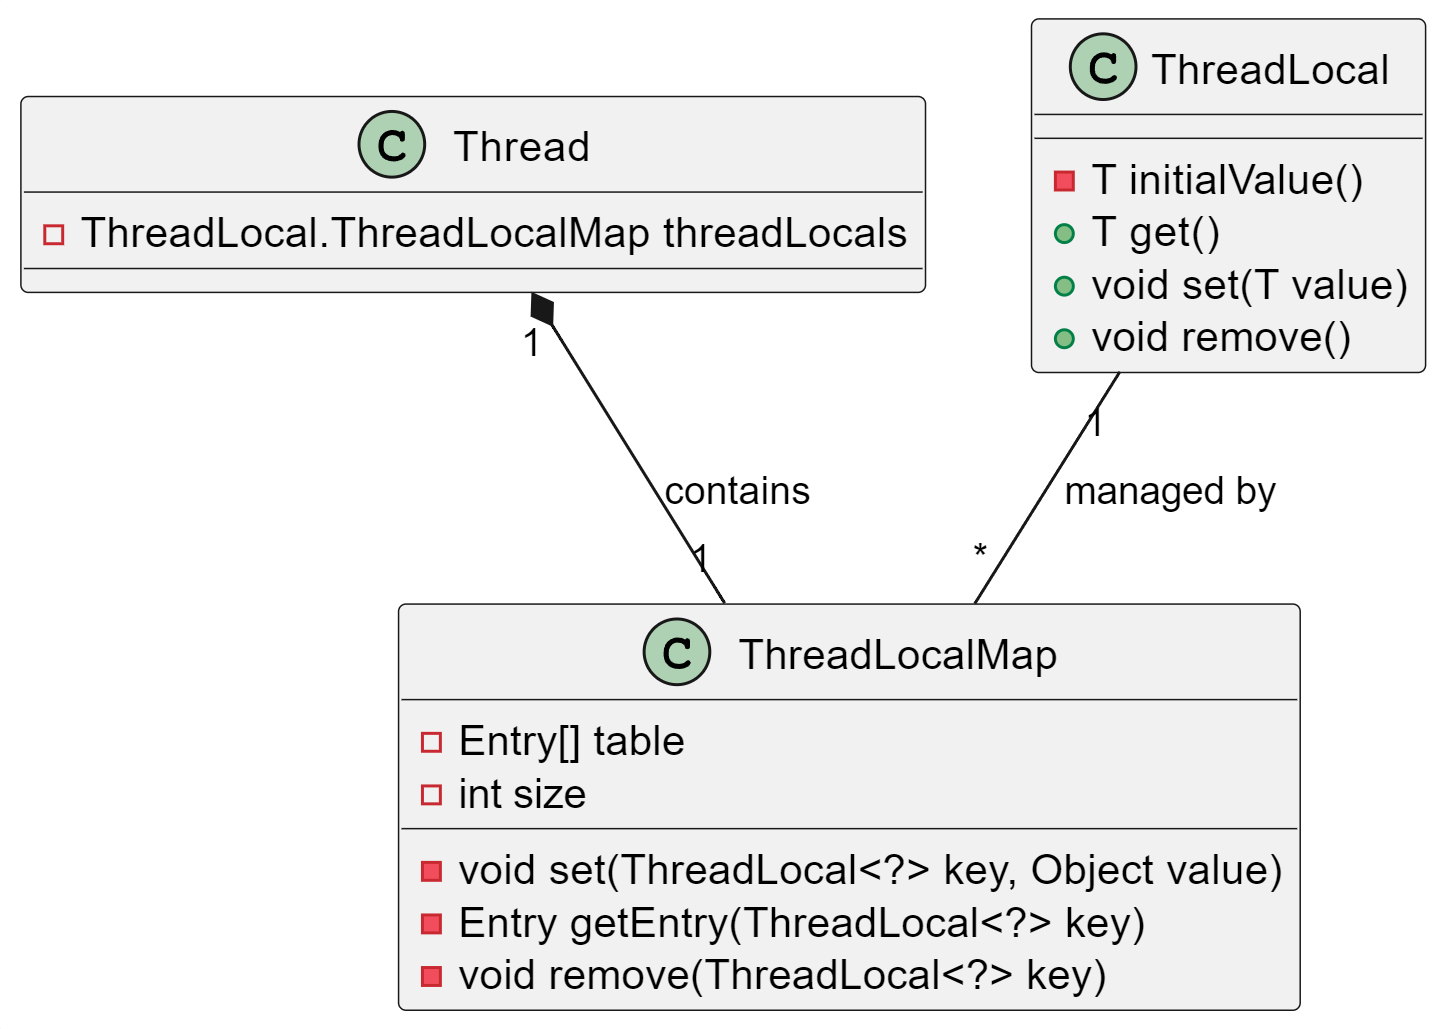
\includegraphics[width=0.6\textwidth]{ThreadLocalUML.png}
        \caption{Überblick Aufbau von ThreadLocal}
        \label{fig:ThreadLocalMap}
    \end{figure}
    Dasselbe gilt auch für \texttt{InheritableTreadLocal}. Wird in einem Thread ein neuer gestartet, erbt dabei aber der Kind-Thread alle Einträge des Eltern-Threads. 
    Ein Vorteil von \Glspl{vt} ist, dass sie wegen ihrer geringeren Kosten in großen Mengen verfügbar sind und erstellt werden können. Dabei können sich die Eigenschaften von \texttt{ThreadLocal}
    als Problem herausstellen. Vor allem bei großen Variablen kann dies zu einem sehr hohen Speicherbedarf führen. Bei \texttt{InheritableThreadLocal} kann die Allokation des Speichers
    für die Vererbung zusätzlich einen großen Verwaltungsaufwand bewirken. 

    \texttt{ScopedValue} hingegen ist wie ein Behälter-Objekt, das den tatsächlichen Datenwert und den Zugriff darauf verwaltet. Die Methode \texttt{get()} sucht beim initialen Aufruf nach
    der Wertbindung des innersten Gültigkeitsbereichs. Dabei werden die Ergebnisse in einem kleinen Cache des Threads zwischengespeichert. Dadurch werden nachfolgenden Aufrufe der
    Methode stark beschleunigt. Übersteigt die Menge an bereichsgebundenen Variablen die Größe des Cache, leidet die Geschwindigkeit stark daran. Die Größe beträgt normalerweise 16 Einträge
    und lässt sich mit der \gls{jvm}-Option \texttt{-Djava.lang.ScopedValue.cacheSize=<newSize>} auf eine Größe von 2 bis 16 in 2er-Potenzen verändern. Dabei muss ein Kompromiss
    zwischen Speicherbedarf und Geschwindigkeit gefunden werden. Werden mehr Werte benötigt, kann es sinnvoll sein, sie in einem Record zusammenzufassen und so an eine Instanz von ScopedValue
    zu binden. 

    Wie bereits vorher erwähnt, ist die Vererbung bei \texttt{TreadLocal} speicher- und laufzeitintensiv, da alle Einträge der \texttt{ThreadlocalMap} in den neuen Thread kopiert werden müssen.
    Bei \texttt{ScopedValue} wird dieser Vorgang nicht benötigt. Dadurch fällt viel an Verwaltungsaufwand weg. 

    Bei \texttt{ThreadLocal} wird, wenn einmal mit der \texttt{set}-Methode gesetzt, die Lebensdauer des Wertes nur durch die Lebensdauer des Threads begrenzt und sollte immer mit dem Methodenaufruf
    \texttt{remove} wieder freigegeben werden. Bei langlebigen Threads kann dies zu nicht notwendigen Speicherbedarf führen. Bei Verwendung eines Threadpools -- vor allem eines \emph{newCachedThreadPool} -- 
    können bestehende \Glspl{pt}, falls verfügbar, wiederverwendet werden. Diese Vorgehen kann zwar die Geschwindigkeit des Programms erhöhen, jedoch können dadurch auch Variablen,
    wenn nicht manuell entfernt, in eine andere Aufgabe gelangen und so eine potentielle Sicherheitslücke darstellen. Der \emph{Garbage-Collector} kann die Variable nicht freigeben, da sie noch über 
    den Thread also einer \emph{GC-Root} erreichbar bleibt. Bei \texttt{ScopedValue}s hingegen ist die Lebenszeit an den Gültigkeitsbereich, der als \texttt{Runnable} der \texttt{run}-Methode mitgegeben wird,
    gebunden. Dadurch wird der Wert unzugänglich, wenn der Gültigkeitsbereich wieder verlassen wird. Eine manuelle Entfernung durch einen Methodenaufruf ist nicht nötig.

    Einen weiteren Unterschied stellt die Veränderbarkeit der Variablen dar. \texttt{Thread\-Local}-Variablen sind uneingeschränkt mit der \texttt{set} Methode veränderbar.
    Auch die Verwendung der Schlüsselwortes \texttt{final} schützt nicht davor. Dadurch wird ein Datenfluss in alle Richtungen zwischen Methoden gewährleistet. Dies kann zu sehr unübersichtlichen 
    Kommunikationsfluss in Form von sogenannten "Spaghetti-Code" führen. Die Klasse \texttt{ScopedValue} hingegen lässt einen Datenfluss nur in eine Richtung zu. Der Wert kann innerhalb des 
    Gültigkeitsbereichs durch einen neuen verschachtelten Gültigkeitsbereich überschrieben werden. Diese Änderung ist aber nicht mehr außerhalb des neuen Bereichs sichtbar und ist damit im Aufrufstapels weiter
    unten nicht gültig \cite{JEP481}.
    \begin{program} [H]
        \caption{ThreadLocal}
        \label{prog:ThreadLocal}
    \begin{JavaCode}[language=Java, numbers=left]
static ThreadLocal<String> threadLokal = new ThreadLocal<>();
public static void main(String[] args) {
    threadLokal.set("the negative side of Threadlocal");
    printHello();
    System.out.println(STR."This is a Methode to show \{threadLokal.get()}");
    threadLokal.remove();
}

public static void printHello() {
    threadLokal.set(Thread.currentThread().toString());
    System.out.println(STR."Hello from \{threadLokal.get()}");
}\end{JavaCode}
    \end{program}
    In Programm \ref{prog:ThreadLocal} in Zeile 3 wird der Wert der thread-lokalen Variable gesetzt. In Zeile 4 wird eine Methode aufgerufen, die den Wert aus diversen Gründen überschreibt. Die Wertabfrage in Zeile 5
    retourniert den zuletzt gesetzten Wert, auch wenn dies in einer anderen Methode geschieht. Das Verhalten von \texttt{ScopedValue} kann in Programm \ref{prog:VerwendungVonSV} beobachtet werden.


